\documentclass[swedish]{article}

\usepackage[a4paper,left=1in,right=1in,top=1.25in,bottom=1.25in]{geometry}
\usepackage[style=iso]{datetime2}
\usepackage{graphicx}
\usepackage{amssymb}
\usepackage{amsmath}
\usepackage{mathtools}

\author{Arvid Karlgren}
\title{Föreläsning 1\\
       \LARGE Gränsvärden: Definition och räkneregler}
\date{2023-01-16}

\renewcommand{\contentsname}{Innehåll}
\setlength\parindent{0pt}

\begin{document}

\maketitle

%\tableofcontents

\pagebreak

\section{Kursens mål}

Kursen kommer att hantera följande områden:

\begin{enumerate}
    \item Kontinuitet
    \item Gränsvärden
    \item Derivata
    \item Funktionsundersökning
    \item Primitiva funktioner
    \item Integraler
\end{enumerate}

\pagebreak

\section{Gränsvärden}

\subsection{Definition}

Gränsvärden handlar om hur en funktion ser ut (vilka värden den antar) när x närmar sig olika värden. Det finns två typer av gränsvärden.

\begin{itemize}
    \item{Nära (men ej i) en punkt $a\in x$.}
    \item{För obegränsat stora positiva eller negativa $x\in \mathbb{R}$.}
\end{itemize}

Gränsvärden betecknas med $\to$, till exempel $x \to a$ ("$x$ går mot $a$").

Figur 1 visar några fall där den exakta definitionen av gränsvärden spelar stor roll. 

\begin{figure}[h!]
    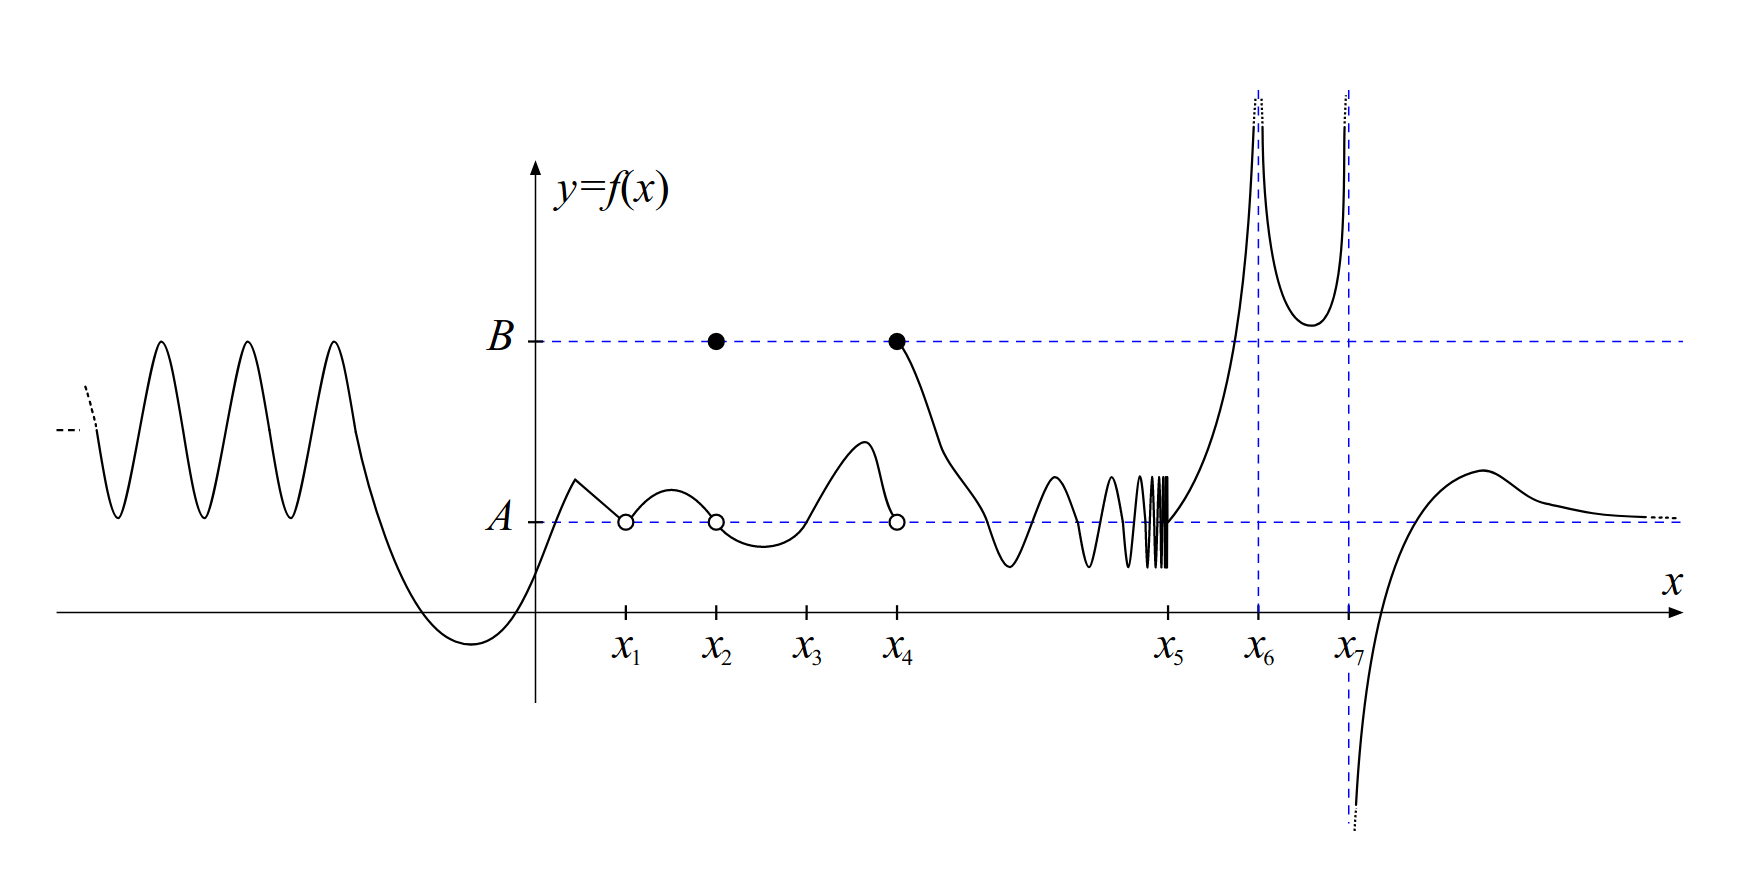
\includegraphics[width=\linewidth]{figur1.png}
    \label{fig:figur1}
    \caption{Olika fall för gränsvärden.}
\end{figure}

Utifrån figur 1 vill vi, utifrån definitionen för gränsvärden, kunna säga följande:

\begin{itemize}
    \item{$f(x) \to A$ då $x \to x_1$, ($x_1 \notin D_f$), skrivs $\lim\limits_{x \to x_1} f(x) = A$}
    \item{$f(x) \to A$ då $x \to x_2$, ($x_2 \in D_f$, $f(x_2) = B$).}
    \item{$f(x) \to A$ då $x \to x_3$, ($x_3 \in D_f$, $f(x_3) = A$).}
    \item{$f(x)$ saknar gränsvärden då $x \to x_4$ eller $x \to x_5$, skrivs $\lim\limits_{x \to x_4} f(x) \; \nexists$}
        \begin{itemize}
            \item{Däremot:
                \smallbreak
                $\lim\limits_{x \to x_4^-} = A \quad$ (Vänstergränsvärde, från vänster)\\

                $\lim\limits_{x \to x_4^+} = B \quad$ (Högergränsvärde, från höger)}
        \end{itemize}
    \smallbreak
    \item{$f(x) \to \infty$ då $x \to x_6$}
    \item{$f(x)$ saknar gränsvärde då $x \to x_7$}
    \item{$f(x) \to A$ då $x \to \infty$}
    \item{$f(x)$ saknar gränsvärde då $x \to -\infty$}
\end{itemize}

\bigbreak

{\large\underline{$x \to a$}}

\smallbreak

\textbf{Definition:}

\smallskip

Gränsvärdet för $x \to a$ blir $A$, dvs. $\lim\limits_{x \to a} = A$ om det till varje $\epsilon < 0$ finns ett $\delta < 0$ sådant att $|f(x) - A| < \epsilon$ om $x \in D_f$ och $0 < |x - a| < \delta$ (se figur 2 nedan). 

\begin{figure}[h!]
    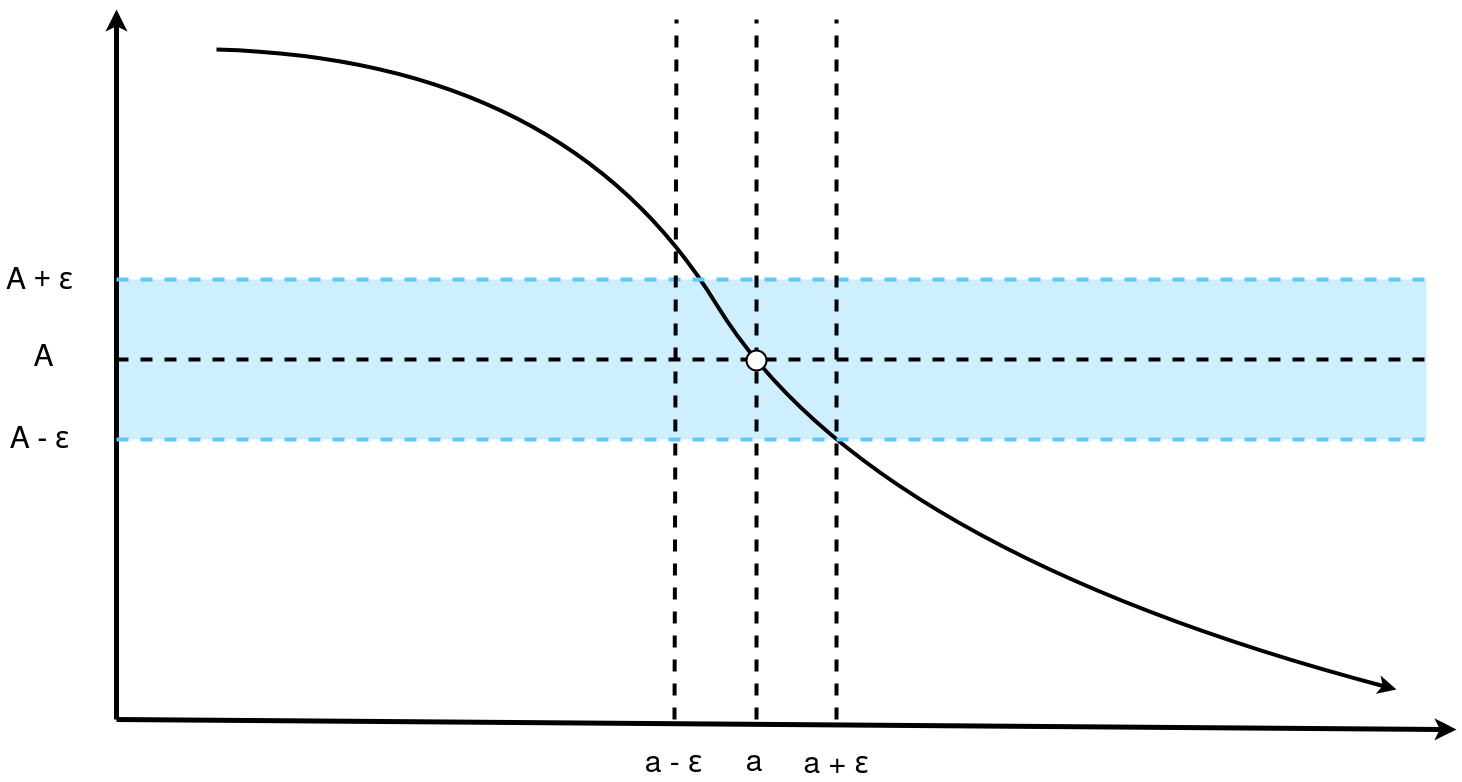
\includegraphics[width=14cm]{figur2.png}
    \label{fig:figur2}
    \caption{Definition av $x \to a$.}
\end{figure}

{\large\underline{$x \to \infty$}}

\smallbreak

\textbf{Definition:}

Gränsvärdet för $x \to \infty$ blir $A$ om det till varje $\epsilon < 0$ finns ett $\omega$ sådant att $|f(x) - A| < \epsilon$ om $x \in D_f$ och $x > \omega$. \textbf{OBS!} krav finns på $D_f$, se boken. 

\begin{figure}[h!]
    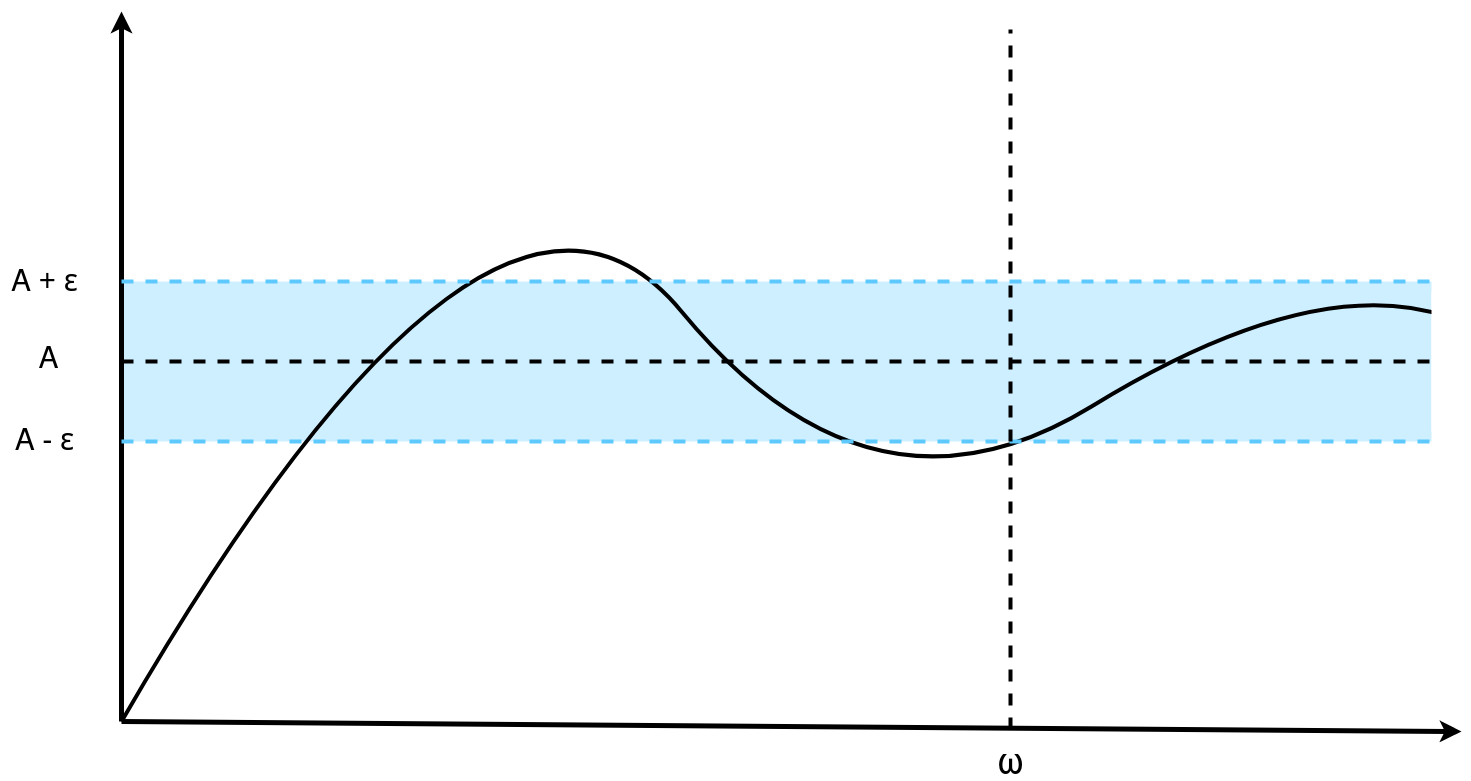
\includegraphics[width=14cm]{figur3.png}
    \label{fig:figur3}
    \caption{Definition av $x \to a$.}
\end{figure}

\subsubsection{Exempel 1}

\textbf{Visa att $\sqrt{x} \to \sqrt{a}$ då $x \to a$ och $a > 0$.}

Låt $\epsilon > 0$. Vi ska hitta passande $\delta$.

\[|\underbrace{\sqrt{x}}_{f(x)} - \underbrace{\sqrt{a}}_A| = \left|\frac{x-a}{\sqrt{x}+\sqrt{a}}\right| \leq \left|\frac{x-a}{\sqrt{a}}\right| = \frac{1}{\sqrt{a}} \cdot \left| x - a \right|\]

\bigbreak

så om $\frac{1}{\sqrt{a}} < |x-a| < \epsilon$ , dvs om $0 < |x-a| < \epsilon \cdot \sqrt{a}$ , så är $|\sqrt{x} - \sqrt{a} | < \epsilon$

\bigbreak

Vi har alltså till varje $\epsilon < 0$ hittat ett $\delta \; (\delta = \epsilon \cdot \sqrt{a})$ så vo har visat att $\lim\limits_{x \to a} = \sqrt{a}$.

\subsubsection{Exempel 2}

$\lim\limits_{x\to \infty}$ existerar ej ty $sin(n\pi) = 0$ och $sin\left(\frac{\pi}{2} + n2\pi \right) = 1$, $n\in \mathbb{R}$.

\subsubsection{Exempel 3}

\begin{itemize}
    \item{\; $\lim\limits_{x\to \infty} \frac{1}{x^n} = 0$,\; $n = 1,\; 2,\; 3...$}
    \item{\; $\lim\limits_{x\to \infty} x^n = \infty$,\; $n = 1,\; 2,\; 3...$}
    \item{$\left. \begin{array}{l}
    \lim\limits_{x\to 0^-} \frac{1}{x} = \infty\\
    \\
    \lim\limits_{x\to 0^-} \frac{1}{x} = \infty
    \end{array} \right\}$} $\lim\limits_{x\to 0} \; \frac{1}{x} \; \nexists$
\end{itemize}


\subsection{Räkneregler}

\begin{itemize} 
    \item{\textbf{Sats 1:} $\left\{ \begin{array}{l}
            f(x) \to 0 \text{ då } x \to a\\
            \\
            g(x) \text{ är begränsad.}
    \end{array} \right. \; \Rightarrow \; f(x) \cdot g(x) \to 0 \text{ då } x \to a$}
        \begin{itemize}    
            \item{$A, \; B\in \mathbb{R}$ och $\; a$ kan bytas mot $a^-, \; a^+, \; - \infty, \ \infty$.}
            \item{"Begränsad" innebär att det finns ett stort tal $C$ sådant att $|g(x)| < C$ i $D_g$.}
        \end{itemize}
    \item{\textbf{Sats 2:} $\left\{ \begin{array}{l}
            f(x) \to A\\
            \\
            g(x) \to B
    \end{array} \right. \text{ då } x \to a \; \Rightarrow \left\{ \begin{array}{l}
            f(x) \pm g(x) \to A \pm B\\
            \\
            f(x) \cdot g(x) \to A \cdot B\\
            \\
            \frac{f(x)}{g(x)} \to \frac{A}{B} \textbf{ endast om $B \neq 0$}
        \end{array} \right.$}
        \bigbreak
    \item{\textbf{Sats 3:} $\left\{ \begin{array}{l}
            f(x) \to A\\
            \\
            g(x) \to \infty
    \end{array} \right. \text{ då } x \to a \; \Rightarrow \; f(x) \cdot g(x) \to \left\{ \begin{array}{l}
        \infty \text{ om } A>0\\
        \\
        - \infty \text{ om } A<0 \text{ då } x \to a\\
        \\
        \text{oklart om } A = 0
    \end{array} \right.$}
\item{Se även sats 3.3 och 3.4 i boken.}

\end{itemize}

\subsection{Räkne-exempel}

Lösta exempel på lösta gränsvärden enligt teori räkneregler ovan. 

\subsubsection{Exempel 4}

Vad blir $\lim\limits_{x \to 1} \; \frac{x^2 + 2x - 3}{x^2 - 1} = $ ?

\smallbreak

Notera att detta gränsvärde är av typen $\left[ \frac{0}{0} \right]$.

$$\frac{x^2 + 2x - 3}{x^2 - 1} = \frac{(x-1)(x+3)}{(x-1)(x+1)} = \frac{x+3}{x+1} \; \xrightarrow{\text{Sats 2}} \; \frac{1+3}{1+1} = 2 \; \text{ då } \; x \to 1$$

Alltså blir $\lim\limits_{x \to 1} f(x) = 2$

\subsubsection{Exempel 5}

Vad blir $\lim\limits_{x \to \infty} \frac{4x^2 - 3x}{17-5x^2} =$ ?

\smallbreak

Detta gränsvärde är av typen $\left[ \frac{\infty + \infty}{- \infty} \right]$

$$\frac{4x^2 - 3x}{17-5x^2} = \frac{x^2(4-\frac{3}{x})}{x^2(\frac{17}{x^2}-5)} = \frac{4-\frac{3}{x}}{\frac{17}{x^2} - 5} \; \to \; \frac{4 - 0}{+ - 5} = -\frac{4}{5} \; \text{ då } \; x \to \infty$$

\subsubsection{Exempel 6}

Vad blir $\lim\limits_{x \to \infty} \; \frac{x - x^3}{x^2 + x} =$ ?

\bigbreak

$$\frac{x-x^3}{x^2+x} = \frac{x^3(\frac{1}{x^2}-1)}{x^2(1+\frac{1}{x})} = \underbrace{x}_{\to \infty} \cdot \underbrace{\frac{\frac{1}{x^2}-1}{1+\frac{1}{x}}}_{\to \frac{0-1}{1+0} = -1} \; \xrightarrow{\text{Sats 3}} \; - \infty \text{ då } x \to \infty$$

\subsubsection{Exempel 7}

Vad händer när ett gränsvärde är av typen $\left[ 0 \cdot \infty \right]$ ?

\bigbreak

$\left\{ \begin{array}{l}
    \frac{17}{x^2} \cdot x = \frac{17}{x} \to 0 \text{ då } x \to \infty\\
    \\
    \frac{17}{x^2} \cdot x^2 = 17 \to 17 \text{ då } x \to \infty\\ 
    \\
    \frac{17}{x^2} \cdot x^3 = 17x \to \infty \text{ då } x \to \infty
\end{array} \right.$

\bigbreak

\textbf{Svar: } Det beror på.

\subsubsection{Exempel 8}

Vad blir $\lim\limits_{x \to \infty} \frac{1 + 2sinx}{x}$ ?

\bigbreak

Notera att sats 2 inte fungerar, eftersom $2sinx$ inte har något gränsvärde. 

$$\frac{1+2sinx}{x} = \underbrace{\frac{1}{x}}_{\to 0} \underbrace{(1+2sinx)}_{\text{Begränsad}} \xrightarrow{\text{Sats 1}} 0 \text{ då } x \to \infty$$

\end{document}
